\documentclass{article}

\usepackage{tikz}
\usetikzlibrary{arrows}
\usetikzlibrary{calc}

\begin{document}

%Without Transparency:
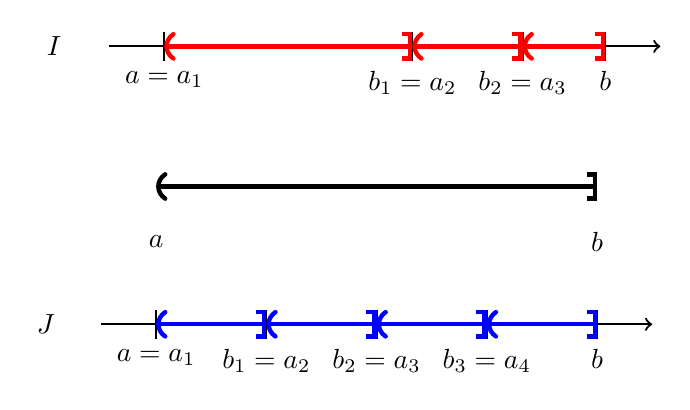
\begin{tikzpicture}[scale=7]
    \begin{scope}[local bounding box=scope1]
	\draw[->, thick] (-0.1,0) -- (0.9,0);
	\node at (-0.2,0) {$I$};
	\foreach \x/\xtext in {0/$a=a_1$,0.45/$b_1=a_2$,0.65/$b_2=a_3$,0.8/$b$}
	\draw[thick] (\x,0.75pt) -- (\x,-0.75pt) node[below] {\xtext};
	\draw[[-), ultra thick, red] (0.45,0) -- (0,0);
	\draw[[-), ultra thick, red] (0.65,0) -- (0.45,0);
	\draw[[-), ultra thick, red] (0.8,0) -- (0.65,0);
    \end{scope}
    \begin{scope}[shift={($(scope1.south)+(-0.35,-0.40cm)$)}]
	\draw[->, thick] (-0.1,0) -- (0.9,0);
	\node at (-0.2,0) {$J$};
	\foreach \x/\xtext in {0/$a=a_1$,0.2/$b_1=a_2$,0.4/$b_2=a_3$,0.6/$b_3=a_4$,0.8/$b$}
	\draw[thick] (\x,0.75pt) -- (\x,-0.75pt) node[below] {\xtext};
	\draw[[-), ultra thick, blue] (0.2,0) -- (0,0);
	\draw[[-), ultra thick, blue] (0.4,0) -- (0.2,0);
	\draw[[-), ultra thick, blue] (0.6,0) -- (0.4,0);
	\draw[[-), ultra thick, blue] (0.8,0) -- (0.6,0);
    \end{scope}
    \begin{scope}[shift={($(scope1.south)+(-0.35,-0.15cm)$)}]
	\draw[[-), ultra thick] (0.8,0) -- (0,0);
	\node at (0,-0.1) {$a$};
	\node at (0.8,-0.1) {$b$};
    \end{scope}
\end{tikzpicture}

\end{document}
